\documentclass[11pt]{amsart}
\usepackage{amsfonts,amssymb,amsmath}
\usepackage{xltxtra}
\usepackage{unicode-math}
\setmathfont{Asana-Math.otf}
\usepackage{pstricks-add}
\usepackage{geometry}
\geometry{
 a4paper,
 total={210mm,297mm},
 left=10mm,
 right=10mm,
 top=15mm,
 bottom=15mm,
 }
\setmainfont[Mapping=tex-text]{Garamond Premier Pro}
\usepackage{graphicx}\usepackage{sidecap}\usepackage{bbm}
\title{\textbf{Assignments Of Complex Analysis}\\\textit{instructor Petra 
Bonfert-Taylor}}
\author{George Papadopoulos\\ pgeorgios8@gmail.com\\12th April 2017}
\newcommand{\dsp}{\displaystyle}
\newcommand{\BBC}{\mathbb{C}}\newcommand{\mi}{\mathfrak{i}}
\setlength\parindent{0pt}\usepackage{color,colortbl}
\newcommand{\degre}{\ensuremath{^\circ}}
\usepackage{caption}\usepackage{subcaption}
\begin{document}
\maketitle\[
\includegraphics[scale = 0.25]{wesleyan.png}\]
\section{First Assignment}
\textbf{1.} Graph the following four sets:\\
(A) $\dsp \left\{z\in\BBC\;\left|\; |z-3-2\mi|\leq 1\right.\right\}$\\
(B) $\dsp \left\{z\in\BBC\;\left|\; \mathfrak{Im}(z) = 2\right.\right\}$\\
(C) $\dsp\left\{z\in\BBC\setminus\{0\}\;\left|\;0<\arg{z}<\frac{\pi}{6}\right.\right\}$\\
(D) $\dsp \left\{z\in\BBC\;\left|\; |z-1|<|z|\right.\right\}$
\begin{center}
\textbf{Solution}
\end{center}
In the following figures the \textit{x-axis} is the \textbf{real} axis and the 
\textit{y-axis} the \textbf{imaginary} one.
\begin{center}
\begin{figure}
\begin{subfigure}[t]{0.45\linewidth}
\centering
\newrgbcolor{qqccff}{0 0.8 1}
\psset{xunit=1.0cm,yunit=1.0cm,algebraic=true,dotstyle=o,dotsize=3pt 
0,linewidth=0.8pt,arrowsize=3pt 2,arrowinset=0.25}
\begin{pspicture*}(-1.33,-2.36)(4,3.5)
\psaxes[labelFontSize=\scriptstyle,xAxis=true,yAxis=true,Dx=1,Dy=1,ticksize=-2pt 
0,subticks=2]{->}(0,0)(-1.33,-2.36)(4,3.5)
\pscircle[linewidth=2.8pt,linecolor=qqccff,fillcolor=qqccff,fillstyle=solid,opacity=0.75]
(3,2){1}
\begin{scriptsize}
\psdots[dotsize=5pt 0,dotstyle=*](3,2)
\end{scriptsize}
\end{pspicture*}
\caption{$|z-3-2\mi|\leq 1$ is the \textbf{unit} (r=1) disc (circle+interior) with center 
(3,2).}
\end{subfigure} \hfill
\begin{subfigure}[t]{0.45\linewidth}
\centering
\psset{xunit=1.0cm,yunit=1.0cm,algebraic=true,dotstyle=o,dotsize=3pt 
0,linewidth=0.8pt,arrowsize=3pt 2,arrowinset=0.25}
\begin{pspicture*}(-1.33,-2.36)(4,3.5)
\psaxes[labelFontSize=\scriptstyle,xAxis=true,yAxis=true,Dx=1,Dy=1,ticksize=-2pt 
0,subticks=2]{->}(0,0)(-1.3,-2.3)(4,3.4)
\psplot[linewidth=2pt,linecolor=qqccff]{-1.3}{4}{(--2-0*x)/1}
\end{pspicture*}
\caption{With $\mathfrak{Im}(z)=2$, it is clear that the locus of these z is the line 
y=2.} 
\end{subfigure}\hfill
\begin{subfigure}[t]{0.45\linewidth}
\centering
\newrgbcolor{ccqqcc}{0.8 0 0.8}
\newrgbcolor{xdxdff}{0.49 0.49 1}
\newrgbcolor{fftttt}{1 0.2 0.2}
\psset{xunit=1.0cm,yunit=1.0cm,algebraic=true,dotstyle=o,dotsize=3pt 
0,linewidth=0.8pt,arrowsize=3pt 2,arrowinset=0.25}
\begin{pspicture*}(-1.33,-2.36)(4,3.5)
\psaxes[labelFontSize=\scriptstyle,xAxis=true,yAxis=true,Dx=1,Dy=1,ticksize=-2pt 
0,subticks=2]{->}(0,0)(-1.33,-2.36)(4,3.5)
\pspolygon[linewidth=1.6pt,linestyle=dashed,dash=2pt 
2pt,linecolor=fftttt,fillcolor=fftttt,fillstyle=solid,opacity=0.25](6,0)(0,0)(8.4,4.86)
\pscustom[linewidth=1.6pt,linestyle=dashed,dash=2pt 
2pt,linecolor=ccqqcc,fillcolor=ccqqcc,fillstyle=solid,opacity=0.25]{\parametricplot{0.0}{
0.5235987755982987}{2*cos(t)+0|2*sin(t)+0}\lineto(0,0)\closepath}
\psline[linewidth=1.6pt,linestyle=dashed,dash=2pt 2pt,linecolor=fftttt](6,0)(0,0)
\psline[linewidth=1.6pt,linestyle=dashed,dash=2pt 2pt,linecolor=fftttt](0,0)(8.4,4.86)
\psline[linewidth=1.6pt,linestyle=dashed,dash=2pt 2pt,linecolor=fftttt](8.4,4.86)(6,0)
\begin{scriptsize}
\psdots[dotsize=5pt 0](0,0)
\rput[bl](-0.46,0.32){$A$}
\rput[bl](0.78,0.14){\ccqqcc{$30\textrm{\degre}$}}
\psdots[dotstyle=*,linecolor=xdxdff](6,0)
\rput[bl](6.08,0.12){\xdxdff{$C$}}
\psdots[dotstyle=*,linecolor=blue](8.4,4.86)
\rput[bl](8.48,4.98){\blue{$D$}}
\end{scriptsize}
\end{pspicture*}
\caption{It is the colored (light red) region included between the lines 
    $y= \tan\left(\frac{\pi}{6}\right)$ and y=0 without the point (0,0) and of course 
\textbf{without} the points of the lines mentioned above.} 
\end{subfigure}\hfill
\begin{subfigure}[t]{0.45\linewidth}
\centering
\newrgbcolor{qqzzff}{0 0.6 1}
\psset{xunit=1.0cm,yunit=1.0cm,algebraic=true,dotstyle=o,dotsize=3pt 
0,linewidth=0.8pt,arrowsize=3pt 2,arrowinset=0.25}
\begin{pspicture*}(-1.34,-2.35)(4.01,3.51)
\psaxes[labelFontSize=\scriptstyle,xAxis=true,yAxis=true,Dx=1,Dy=1,ticksize=-2pt 
0,subticks=2]{->}(0,0)(-1.34,-2.35)(4.01,3.51)
\pspolygon[linewidth=2.4pt,linestyle=dashed,dash=1pt 2pt 3pt 2pt 
,linecolor=qqzzff,fillcolor=qqzzff,fillstyle=solid,opacity=0.25](0.5,-2.9)(0.5,5.9)(7,
5.9)(7,-2.9)
\psline[linewidth=2.4pt,linestyle=dashed,dash=1pt 2pt 3pt 2pt 
,linecolor=qqzzff](0.5,-2.9)(0.5,5.9)
\psline[linewidth=2.4pt,linestyle=dashed,dash=1pt 2pt 3pt 2pt 
,linecolor=qqzzff](0.5,5.9)(7,5.9)
\psline[linewidth=2.4pt,linestyle=dashed,dash=1pt 2pt 3pt 2pt 
,linecolor=qqzzff](7,5.9)(7,-2.9)
\psline[linewidth=2.4pt,linestyle=dashed,dash=1pt 2pt 3pt 2pt 
,linecolor=qqzzff](7,-2.9)(0.5,-2.9)
\rput[tl](0.71,2.33){$\dsp \mathfrak{Re}(z) > \frac{1}{2} $}
\begin{scriptsize}
\psdots[dotstyle=*,linecolor=blue](0.5,-2.9)
\rput[bl](0.58,-2.79){\blue{$A$}}
\psdots[dotstyle=*,linecolor=blue](0.5,5.9)
\rput[bl](0.58,5.74){\blue{$B$}}
\psdots[dotstyle=*,linecolor=blue](7,5.9)
\rput[bl](7.08,5.74){\blue{$C$}}
\psdots[dotstyle=*,linecolor=blue](7,-2.9)
\rput[bl](7.08,-2.79){\blue{$D$}}
\end{scriptsize}
\end{pspicture*}
\caption{Raise both sides to the power of two, it is the blue sketched region below 
without the points of the vertical line $x=\frac{1}{2}$.} 
\end{subfigure} 
\end{figure}
\end{center}
\textbf{2.} Find and plot the 6th roots of unity. For this problem you need to submit both 
a graph showing your answer as well as the calculation that led you to this graph. 
\begin{center}
\textbf{Solution}
\end{center}
$\dsp z^6=1\Rightarrow |z|^{6}\mathfrak{e}^{6\mi\theta}=1^{6}\mathfrak{e}^{0\cdot\mi}\Rightarrow 
\begin{cases}|z|=1&\\6\theta=2k\pi\Rightarrow 
\theta=\frac{k\pi}{3}&,k=0,1,2,3,4,5\end{cases}$, so the points we seek are
\[
\left\{(1,0),\left(\cos\left(\frac{\pi}{3}\right),\sin\left(\frac{\pi}{3}\right)\right),
\left(\cos\left(\frac{2\pi}{3}\right),\sin\left(\frac{2\pi}{3}\right)\right),
\left(\cos\left(\pi\right) 
,\sin\left(\pi\right)\right),\left(\cos\left(\frac{4\pi}{3}\right),
\sin\left(\frac{4\pi}{3}\right)\right),\left(\cos\left(\frac{5\pi}{3}\right),
\sin\left(\frac{5\pi}{3}
 \right)\right)\right\}
\]
or 
\[
 \left\{(1,0),\left(\frac{1}{2},\frac{\sqrt{3}}{2}\right),\left(-\frac{1}{2},\frac{\sqrt{3}}{2}\right),(-1,0),
 \left(-\frac{1}{2},-\frac{\sqrt{3}}{2}\right),\left(\frac{1}{2},-\frac{\sqrt{3}}{2}\right)\right\}
\]
An easy way to construct the figure is to take $z_1=1$, draw the point (1,0) and then from that point create a 
\textbf{regular} hexagon of side 1 centered at the origin of the axis, which of course is 
also inscribed in the circle of radius 1 and center (0,0). The six solutions are 
represented by the  points A, B, C, D, E, F which are 
the vertices of this regular hexagon, as seen in the following figure.
\begin{center}
\newrgbcolor{zzttff}{0.6 0.2 1}
\newrgbcolor{ffqqcc}{1 0 0.8}
\psset{xunit=2.14406779661017cm,yunit=2.4210526315789473cm,algebraic=true,dotstyle=o,
dotsize=3pt 0,linewidth=0.8pt,arrowsize=3pt 2,arrowinset=0.25}
\begin{pspicture*}(-1.5,-1.5)(1.5,1.5)
\psaxes[labelFontSize=\scriptstyle,xAxis=true,yAxis=true,Dx=1,Dy=1,ticksize=-2pt 
0,subticks=2]{->}(0,0)(-1.5,-1.5)(1.5,1.5)
\pspolygon[linewidth=2pt,linecolor=ffqqcc,fillcolor=ffqqcc,fillstyle=solid,opacity=0.25]
(-1,0)(-0.5,-0.87)(0.5,-0.87)(1,0)(0.5,0.87)(-0.5,0.87)
\psellipse[linewidth=1.2pt,linestyle=dashed,dash=2pt 2pt,linecolor=zzttff](0,0)(1,1)
\psline[linewidth=2pt,linecolor=ffqqcc](-1,0)(-0.5,-0.87)
\psline[linewidth=2pt,linecolor=ffqqcc](-0.5,-0.87)(0.5,-0.87)
\psline[linewidth=2pt,linecolor=ffqqcc](0.5,-0.87)(1,0)
\psline[linewidth=2pt,linecolor=ffqqcc](1,0)(0.5,0.87)
\psline[linewidth=2pt,linecolor=ffqqcc](0.5,0.87)(-0.5,0.87)
\psline[linewidth=2pt,linecolor=ffqqcc](-0.5,0.87)(-1,0)
\begin{scriptsize}
\psdots[dotsize=5pt 0,dotstyle=*](0,0)
\rput[bl](0.03,0.06){$O$}
\psdots[dotsize=5pt 0,dotstyle=*](-1,0)
\rput[bl](-1.11,-0.09){$D$}
\psdots[dotsize=5pt 0,dotstyle=*](-0.5,-0.87)
\rput[bl](-0.57,-1){$E$}
\psdots[dotsize=5pt 0,dotstyle=*](0.5,-0.87)
\rput[bl](0.52,-1){$F$}
\psdots[dotsize=5pt 0,dotstyle=*](1,0)
\rput[bl](1.02,0.06){$A$}
\psdots[dotsize=5pt 0,dotstyle=*](0.5,0.87)
\rput[bl](0.52,0.92){$B$}
\psdots[dotsize=5pt 0,dotstyle=*](-0.5,0.87)
\rput[bl](-0.48,0.92){$C$}
\end{scriptsize}
\end{pspicture*}
\end{center}
\section{Second Assignment}
\textbf{1.} Find the image of the set $\dsp U = \left\{z\in\mathbb{C}\;
\left|\;\frac{-\pi}{2}\leq\mathfrak{Re}(z)\leq\frac{\pi}{2}\right.\right\}$ 
under the function $f(z) = \sin(z)$. To do so please answer the following questions:\\
a. What is the image of the line segment $\dsp 
L_{1}=\left(\frac{\pi}{2},\frac{\pi}{2}\right)$ (in the real axis) under $f$?\\
b.    What is the image of the imaginary axis $\dsp L_{2}=\left\{\mi y\; \left|\;y \in 
\mathbb{R}\right.\right\}$ under $f$?\\
c.    What is the image of the vertical line $L_{3}=\left\{-\frac{\pi}{2}+\mi y\;\left| \;
y\in\mathbb{R}\right.\right\}$ under $f$?\\
d.    What is the image of the vertical line $\dsp L_{4}=\left\{\frac{\pi}{2}+\mi y 
\left| \;y\in\mathbb{R}\right.\right\}$ under $f$?\\
e.    Given your above observations, what do you guess the image of the set $U$ is under 
$f$?
\begin{center}
 \textbf{Solution}
\end{center}
Before we begin answering the questions we need to do some calculations.
\[
f(z) = \sin(z) = \sin(x+y \mi) = \sin(x)\cos(y\mi) + \sin(\mi y)\cos(x) = \sin(x)\cosh(y) 
+\mi\cdot \cos(x)\sinh(y)\]
so $u(x,y) = \sin(x)\cosh(y)$ and $v(x,y) = \cos(x)\sinh(y)$.\\
a. $L_{1}$ is the line segment $\dsp 
\mathfrak{Re}\left(-\frac{\pi}{2},\frac{\pi}{2}\right)$ in the \textit{z-plane}, so for 
$\dsp x\in\left(-\frac{\pi}{2},\frac{\pi}{2}\right)$ and $y=0$ we get $\dsp 
w(x,0)=\left<u(x,0),v(x,0)\right>=\left<\sin(x),0\right>$ 
and for $\dsp x = \pm\frac{\pi}{2}$, $\dsp w\left(\pm\frac{\pi}{2},0\right) = \pm 1$, $f$
which means that under , $L_{1}$ is mapped
into the line segment $\dsp \mathfrak{Re}(-1,1)$ in the \textit{w-plane}.
\[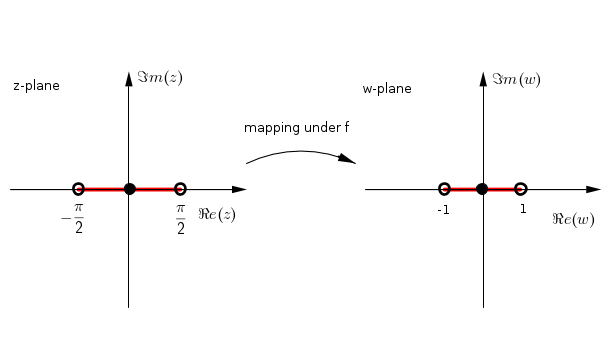
\includegraphics[width = 0.6\linewidth]{1a.png}\]
b. Following the same steps as in answer (a) we get,\[
w(0,y) = \left<u(0,y),v(0,y)\right> = \left<0,\sinh(y)\right>
\]
and since the range of $\sinh$ is $\dsp (-\infty,+\infty)$ for $y\in\mathbb{R}$, we 
deduce that $f$ maps the $y\mi$ line or the 
$\mathfrak{Im}(z)$ axis into the \textit{imaginary} axis $\mathfrak(Im)(w)$ of the 
\textit{w-plane}.
\[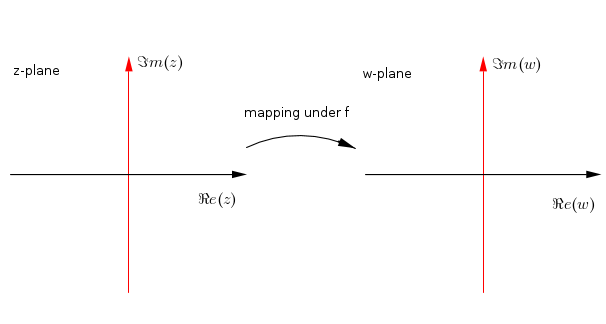
\includegraphics[width = 0.6\linewidth]{1b.png}\]
c. For $\dsp x = -\frac{\pi}{2}$ we get $\dsp 
w\left(-\frac{\pi}{2},y\right)=\left<-\cosh(y),0\right>$ and since the range of $\cosh$ 
is 
$[1,+\infty)$ for $y\in\mathbb{R}$, we deduce that $f$ maps the line $\dsp y = 
-\frac{\pi}{2} + y \mi$ of the \textit{z-plane} into the line 
$\dsp \mathfrak{Re}(-\infty,-1]$ of the \textit{w-plane}, we can imagine that an invisible hand bends the two infinite branches of the 
line $\dsp y = -\frac{\pi}{2}+y\mi$ regarding as the center of the infinite vertical line 
the point $\dsp \left(-\frac{\pi}{2},0\right)$ 
leftwards, until both branched become one with the \textit{real axis} and then the same 
force moves the new line's edge horizontally to 
the point (-1,0). We will see the same process in the next question but in the opposite direction.
\[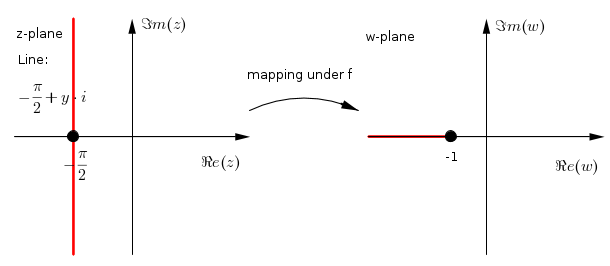
\includegraphics[width = 0.6\linewidth]{1c.png}\]
d. As in (c), $\dsp x = \frac{\pi}{2}$ and so $\dsp w\left(\frac{\pi}{2},y\right)= 
\left<\cosh(y),0\right>$, so $f$ maps the line 
$\dsp y = \frac{\pi}{2} + y \mi$ of the \textit{z-plane} into the line $\dsp \mathfrak{Re}[1,+\infty]$ of the \textit{w-plane}.
\[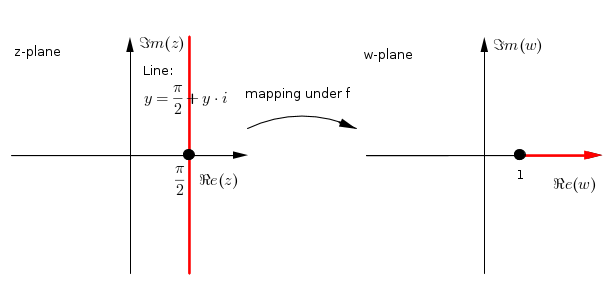
\includegraphics[width = 0.6\linewidth]{1d.png}\]
e. It is clear that $\dsp U = \left\{ z \in 
\BBC\;\left|\;-\frac{\pi}{2}<\mathfrak{Re}(z)<\frac{\pi}{2}\right.\right\}$ is mapped 
into the whole
\textit{w-plane} slit along the rays $\mathfrak{Re}(-\infty,1]$ and $\mathfrak{Re}[1,+\infty)$ (white lines in the next figure excluding
also from the \textit{w-plane} the points (-1,0) and (1,0)).
\[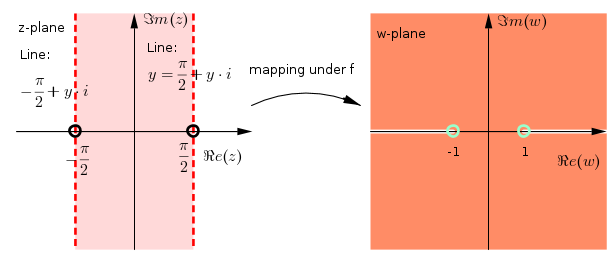
\includegraphics[width = 0.6\linewidth]{1e.png}\]
\textbf{2.} Let $u(x,y) = x^2 - y^2 -y$. Find a real-valued function $v(x,y)$ such that 
$v(0,0)=1$ and together, $u$ and $v$ satisfy the 
\textit{Cauchy-Riemann} equations in the entire complex plane.\\\\
To do so, please follow these steps:\\
a.    Find the partial derivatives $u_x(x,y)$ and $u_y(x,y)$.\\
b.    Using these partial derivatives and the Cauchy-Riemann equations, give equations for the partial derivatives $v_x(x,y)$ and 
$v_y(x,y)$.\\
d.    Find functions $v(x,y)$ that satisfy the equation for the partial derivative with 
respect to $y$.\\
e.    Now find a function $v(x,y)$ that satisfies both equations for the partial 
derivatives at the same time.\\
f.     Finally, check whether the function you found in the previous step satisfies 
$v(0,0)=1$. If not, modify the function so that it does.\\
\begin{center}
\textbf{Solution}
\end{center}
$\dsp u(x,y) = x^2 - y^2 -y$\\
a. $u_{x}(x,y) =2x $ and $u_{y}(x,y) =  -2y - 1$.\\
b. $\dsp \left\{\begin{matrix}u_{x} &=&v_{y} \\ u_{y} &=&-v_{x}\end{matrix}\right.\Rightarrow \left\{\begin{matrix}2x &=&v_{y} \\ -
2y-1 &=&-v_{x}\end{matrix}\right.\Rightarrow \left\{\begin{matrix}v_{y} &=&2x \\ v_{x}&=&2y+1\end{matrix}\right.\Rightarrow 
\left\{\begin{matrix} v_{x}&=&2y+1\\v_{y} &=&2x \end{matrix}\right.$\\
c. From the previous answer we came up with the equation and by integrating with respect 
to $x$ and treating $y$ as a 
\textit{\textbf{constant}} we get,\[v_{x}(x,y)=2y+1\Rightarrow \int v_{x}(x,y)\;\mathbb{d}x = \int 2y +1 \;\mathbb{d}x\Rightarrow v(x,y) =
2xy+x+ay+c \;\;(1)\]
for $a,c\in\mathbb{R}$.\\
d. Following the same process as in (c), but now by integrating with respect to $y$ and 
treating $x$ as a \textit{\textbf{constant}} 
we get \[v_{y}(x,y)=2x \Rightarrow \int v_{y}(x,y)\;\mathbb{d}y = \int 2x \;\mathbb{d}y \Rightarrow v(x,y) = 2xy + bx + d\;\;(2)\]
for $b,d \in \mathbb{R}$.\\
e. Equating relations (1) and (2) from answers c and d respectively we get \begin{eqnarray*}2xy+x+ay+c&=&2xy + bx + d\\ (1-b)x+ay+c-d
&=&0\end{eqnarray*}
so $a=0$, $b=1$ and $c=d$ and $\dsp \boxed{v(x,y)=2xy+x+c}\;\;(3)$.\\
f. From (3) $\dsp v(0,0) = c \Leftrightarrow c = 1 $ for the function $v$ is $v(x,y) = 
2xy+x+1$.
\section{Third Assignment}
\textbf{1.} Sketch the image under the map $f(z)=\textrm{Log}(z)$ of the open half annulus 
$\dsp A=\left\{z\in\BBC\left| 
\mathfrak{e}^{-\frac{\pi}{4}}<|z|<\mathfrak{e}^{\frac{\pi}{4}},\mathfrak{Re}
(z)>0\right.\right\} $.\\Recall: $\textrm{Log}(z)$ denotes the \textit{principal branch} 
of logarithm, that is, $\textrm{Log}(z)=\ln⁡|z|+\mi \textrm{Arg}(z)$, 
where $\dsp -\pi<\textrm{Arg}(z)\leq \pi$ is the principal argument of $z$.\\
The image you create (either by hand or using a computer graphing program) should contain two graphs: On one set of 
coordinate axes, sketch the half annulus $A$, on a second set of axes sketch its image 
under $f$ . Please highlight the following 
parts of your graph:\\
1. The set $\dsp \left\{z\in\BBC\;\left|\;|z| =\mathfrak{e}^{-\frac{\pi}{4}}, 
\mathfrak{Re}(z)>0\right.\right\}$ (this is a part of the boundary
of A) as well as the image of this boundary portion under $f$ in your second graph.\\
2. The set $\dsp \left\{z\in\BBC\;\left|\;|z| 
=\mathfrak{e}^{\frac{\pi}{4}},\mathfrak{Re}(z)>0\right.\right\}$ (this is another part of 
the 
boundary of $A$) as well as the image of this boundary portion under $f$ in your second 
graph (use a different color for these sets 
than you used in the first part if possible).\\
3. The set $\left\{z \in 
\BBC\;\left|\;\mathfrak{e}^{-\frac{\pi}{4}}\leq\mathfrak{Im}(z)\leq\mathfrak{e}^{\frac{\pi
} { 4 } }, \mathfrak{Re}(z)=0\right.\right\}$ (this is yet another part of the boundary 
of $A$) as well as the image of this 
boundary portion under $f$ in your second 
graph (use a third color if possible).\\
4. The set $\dsp \left\{z \in \BBC\;\left|\;-\mathfrak{e}^{\frac{\pi}{4}}\leq 
\mathfrak{Im}(z)\leq-\mathfrak{e}^{-\frac{\pi}{4}},
\mathfrak{Re}(z) = 0\right.\right\}$ (this is the fourth part of the boundary of $A$) as 
well 
as the image of this boundary portion under 
$f$ in your second graph (use a fourth color if possible).\\
5. The set $A$ (on your first graph) and its image $f(A)$ (on your second graph).
\begin{center}
\textbf{Solution}
\end{center}
First of all before we begin with the step by step solution we should always have in our mind that $\dsp\textrm{Log}(z)=\ln|z|+\mi 
\textrm{Arg}(z), for -\pi<\textrm{Arg}(z)\leq \pi$.\\
1. We are given the semicircle $\dsp 
C_{1}=\left\{z\in\BBC\;\left|\;|z|=\mathfrak{e}^{-\frac{\pi}{4}},\mathfrak{Re}
(z)>0\right.\right\}$ and we 
will find its image under $\dsp f(z)=\textrm{Log}(z)$. So for every $z\in C_{1}$we have 
$\dsp \textrm{Arg}(z)\in\left(-\frac{\pi}{2},\frac{\pi}{2}\right)$ and $\text{Log}(z)=\ln(e)-\frac{\pi}{2}+\mi\textrm{Arg}(z)$ so f maps $C_1$ 
into the vertical line $z=-\frac{\pi}{4}+\mi\textrm{Arg}(z)$  of the \textit{w-plane} as seen in the next figure (red semicircle without 
the ending points).
\begin{center}
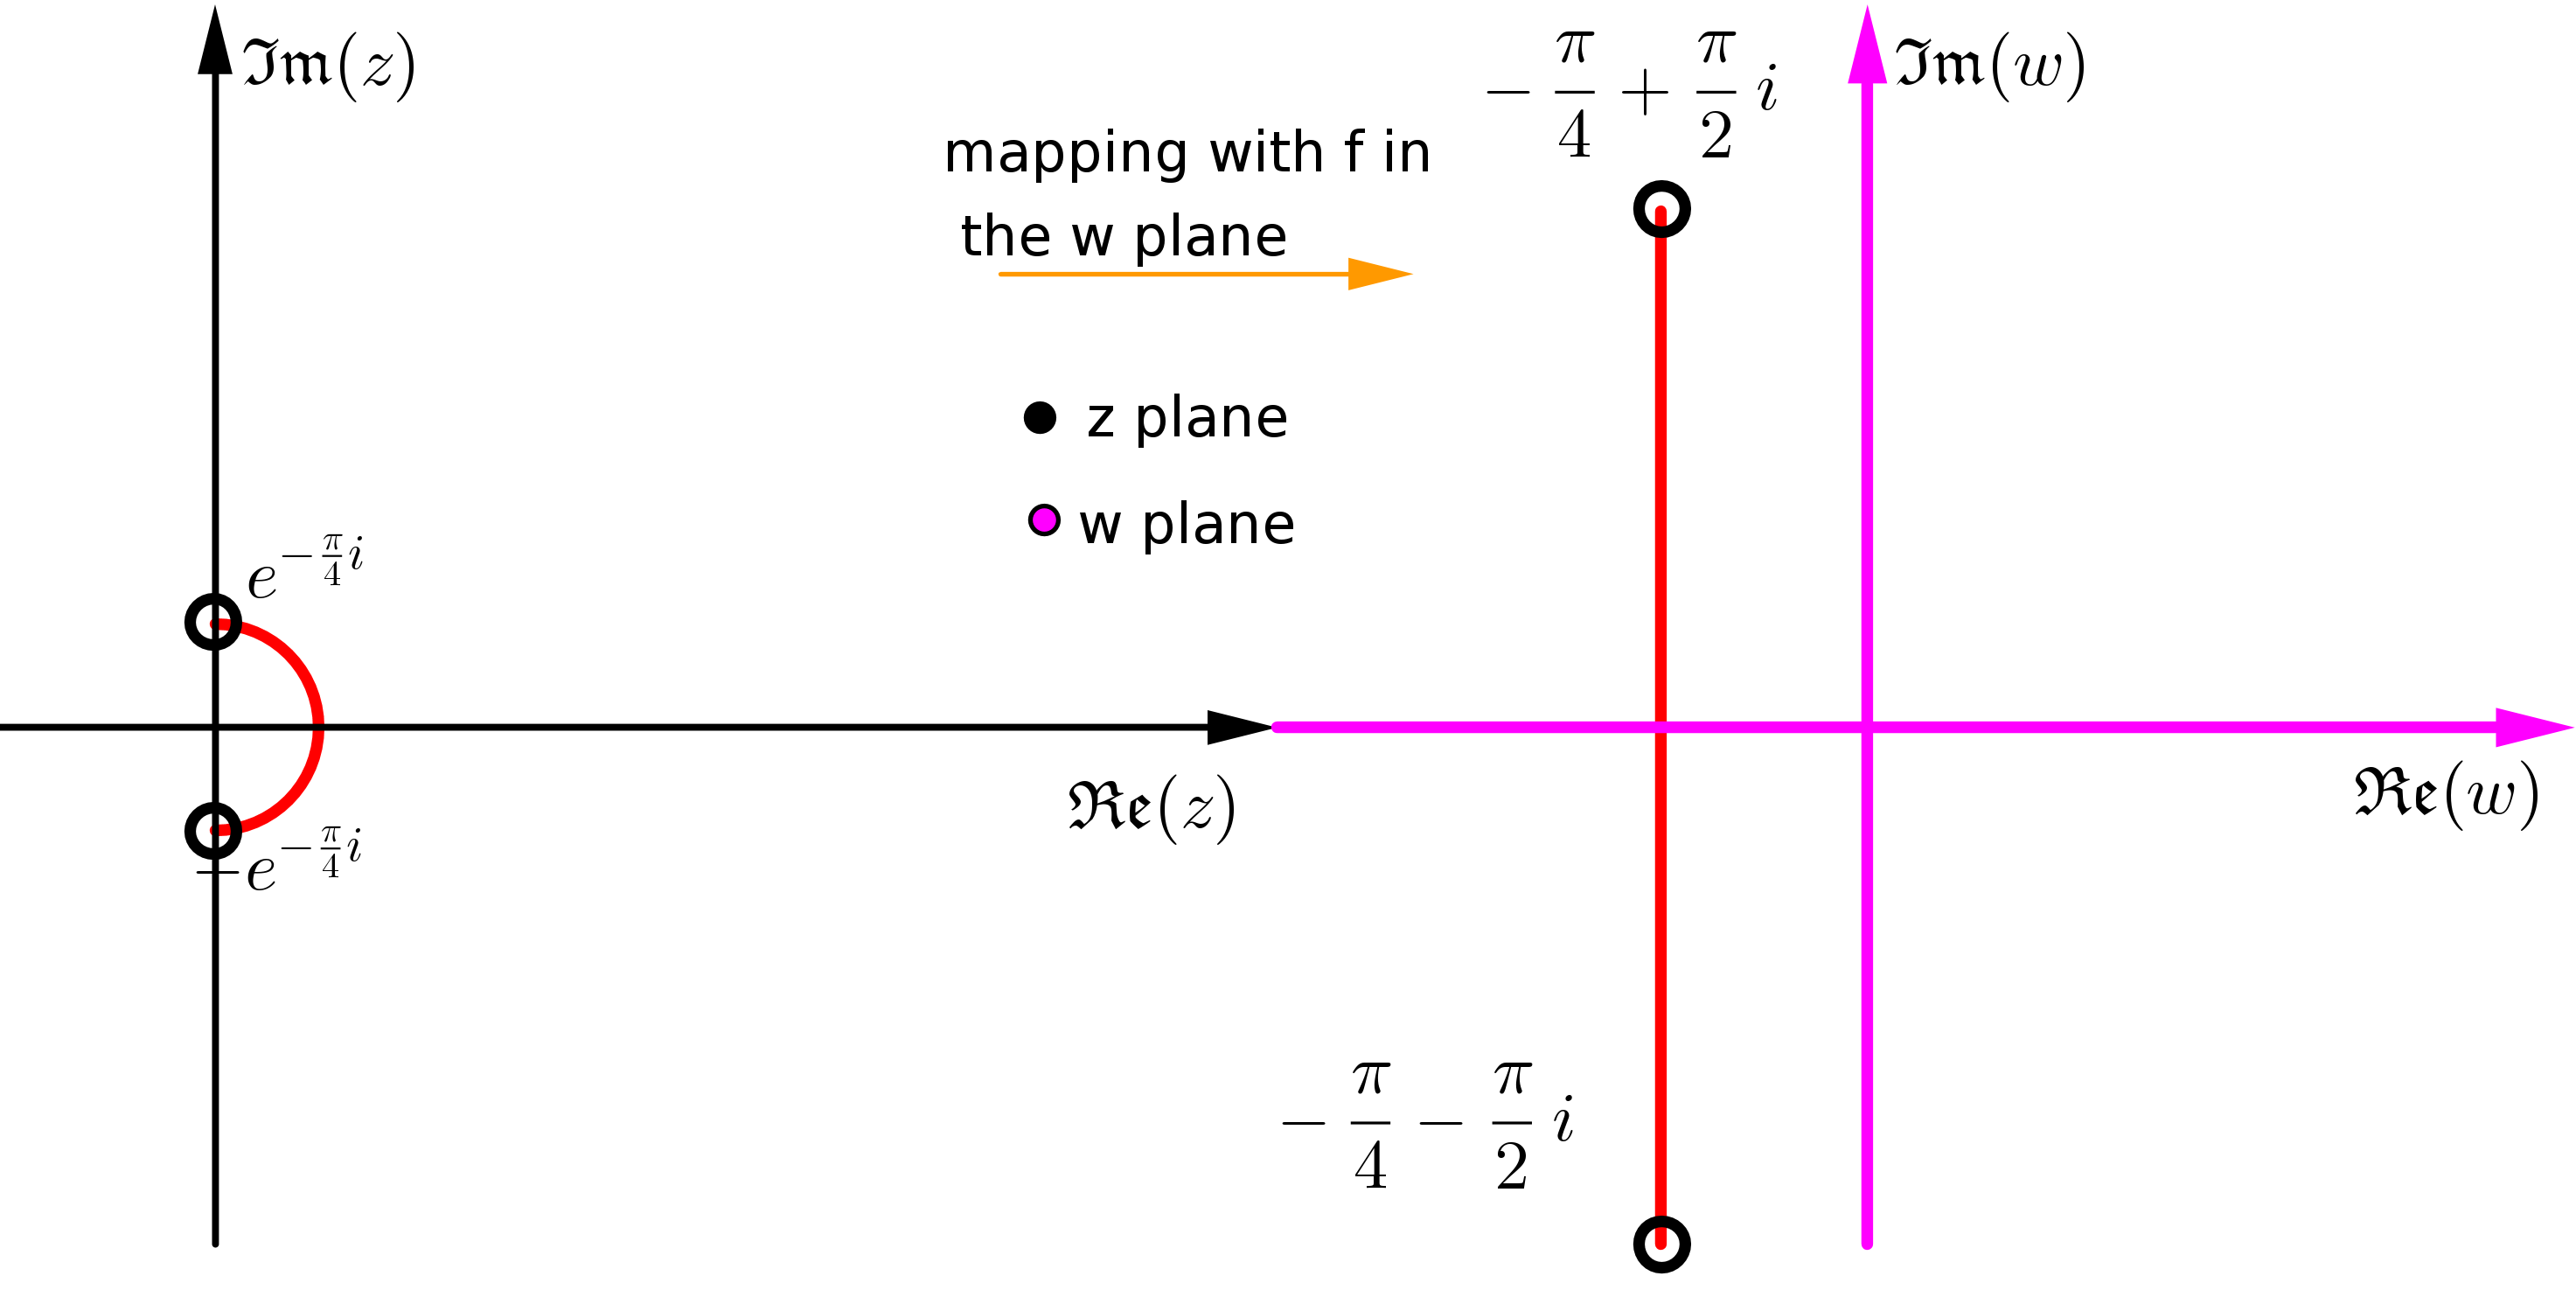
\includegraphics{2a.png}
\end{center}
2. We are given the semicircle $\dsp 
C_{2}=\left\{z\in\BBC\;\left|\;|z|=\mathfrak{e}^{\frac{\pi}{4}},\mathfrak{Re}
(z)>0\right.\right\}$ and 
following the same steps as in (1) we get \[\textrm{Log}(z)=\ln\left(\mathfrak{e}^{\frac{\pi}{4}}\right)+\mi\textrm{Arg}(z)=
\frac{\pi}{4}+\mi\textrm{Arg}(z)\] with $\textrm{Arg}(z)\in\left(-\frac{\pi}{2},\frac{\pi}{2}\right)$. So the blue semicircle $C_2$ without its 
ending points is mapped into the vertical blue line $\dsp z=\frac{\pi}{4}+\mi\textrm{Arg}(z)$ of the \textit{w-plane} without its ending 
points as seen in the next figure.
\begin{center}
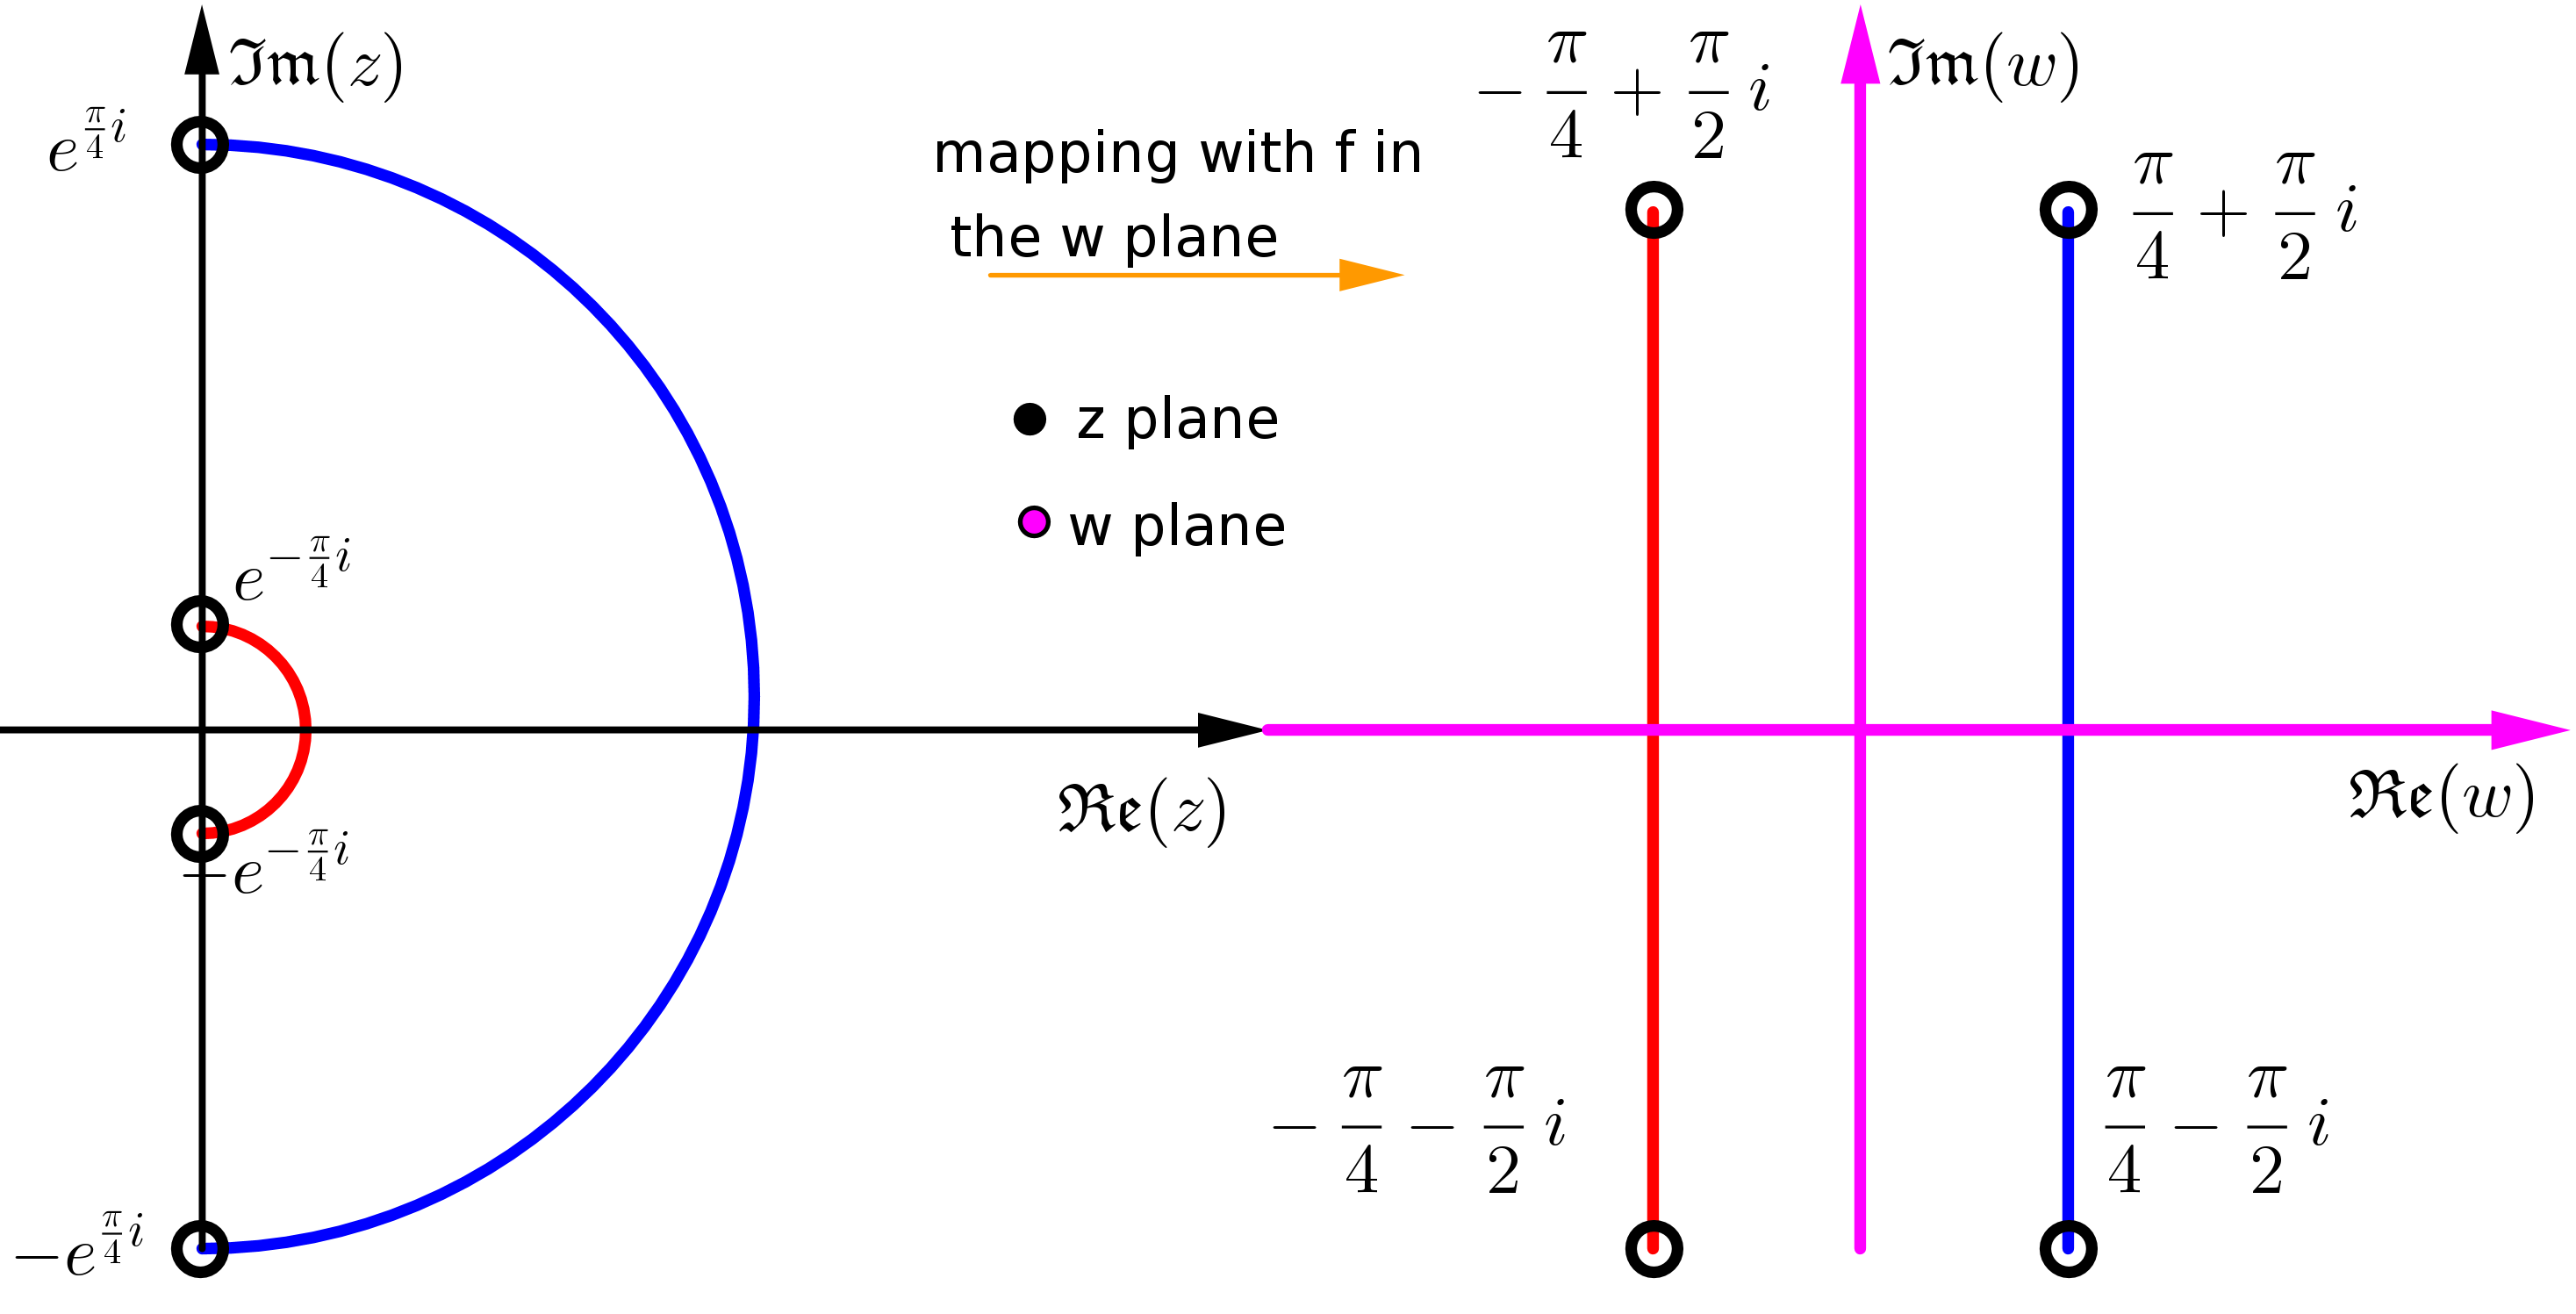
\includegraphics{2b.png}
\end{center}
3. The set $\dsp
C_3=\left\{z\in\BBC\;\left|\;\mathfrak{e}^{-\frac{\pi}{4}}\leq\mathfrak{Im}
(z)\leq\mathfrak { e } ^ {\frac{\pi}{4}}, \
\mathfrak{Re}(z)=0\right.\right\}$ is the vertical line segment which lies in the 
imaginary axis of the \textit{z-plane} with ending points (included)
$\dsp z=\mathfrak{e}^{-\frac{\pi}{4}}\mi$ and $z=\mathfrak{e}^{\frac{\pi}{4}}\mi$. In this case $\dsp\textrm{Arg}(z)=\frac{\pi}{2}$ and 
$\dsp\mathfrak{Re}(z)=0$, so \[\textrm{Log}(z)=\ln|y\cdot \mi|+\frac{\pi}{2}\mi=\ln⁡(y)+\mi\frac{\pi}{2}\] which means that that the 
closed line segment $C_3$ is mapped under $f$ into the closed horizontal line line 
segment $\dsp t+\mi\frac{\pi}{2}$ with 
$t\in\left[-\frac{\pi}{4},\frac{\pi}{2}\right]$. In the next figure we see the orange closed vertical line segment $C_3$ mapped into the 
orange closed horizontal line segment of the \textit{w-plane}.
\begin{center}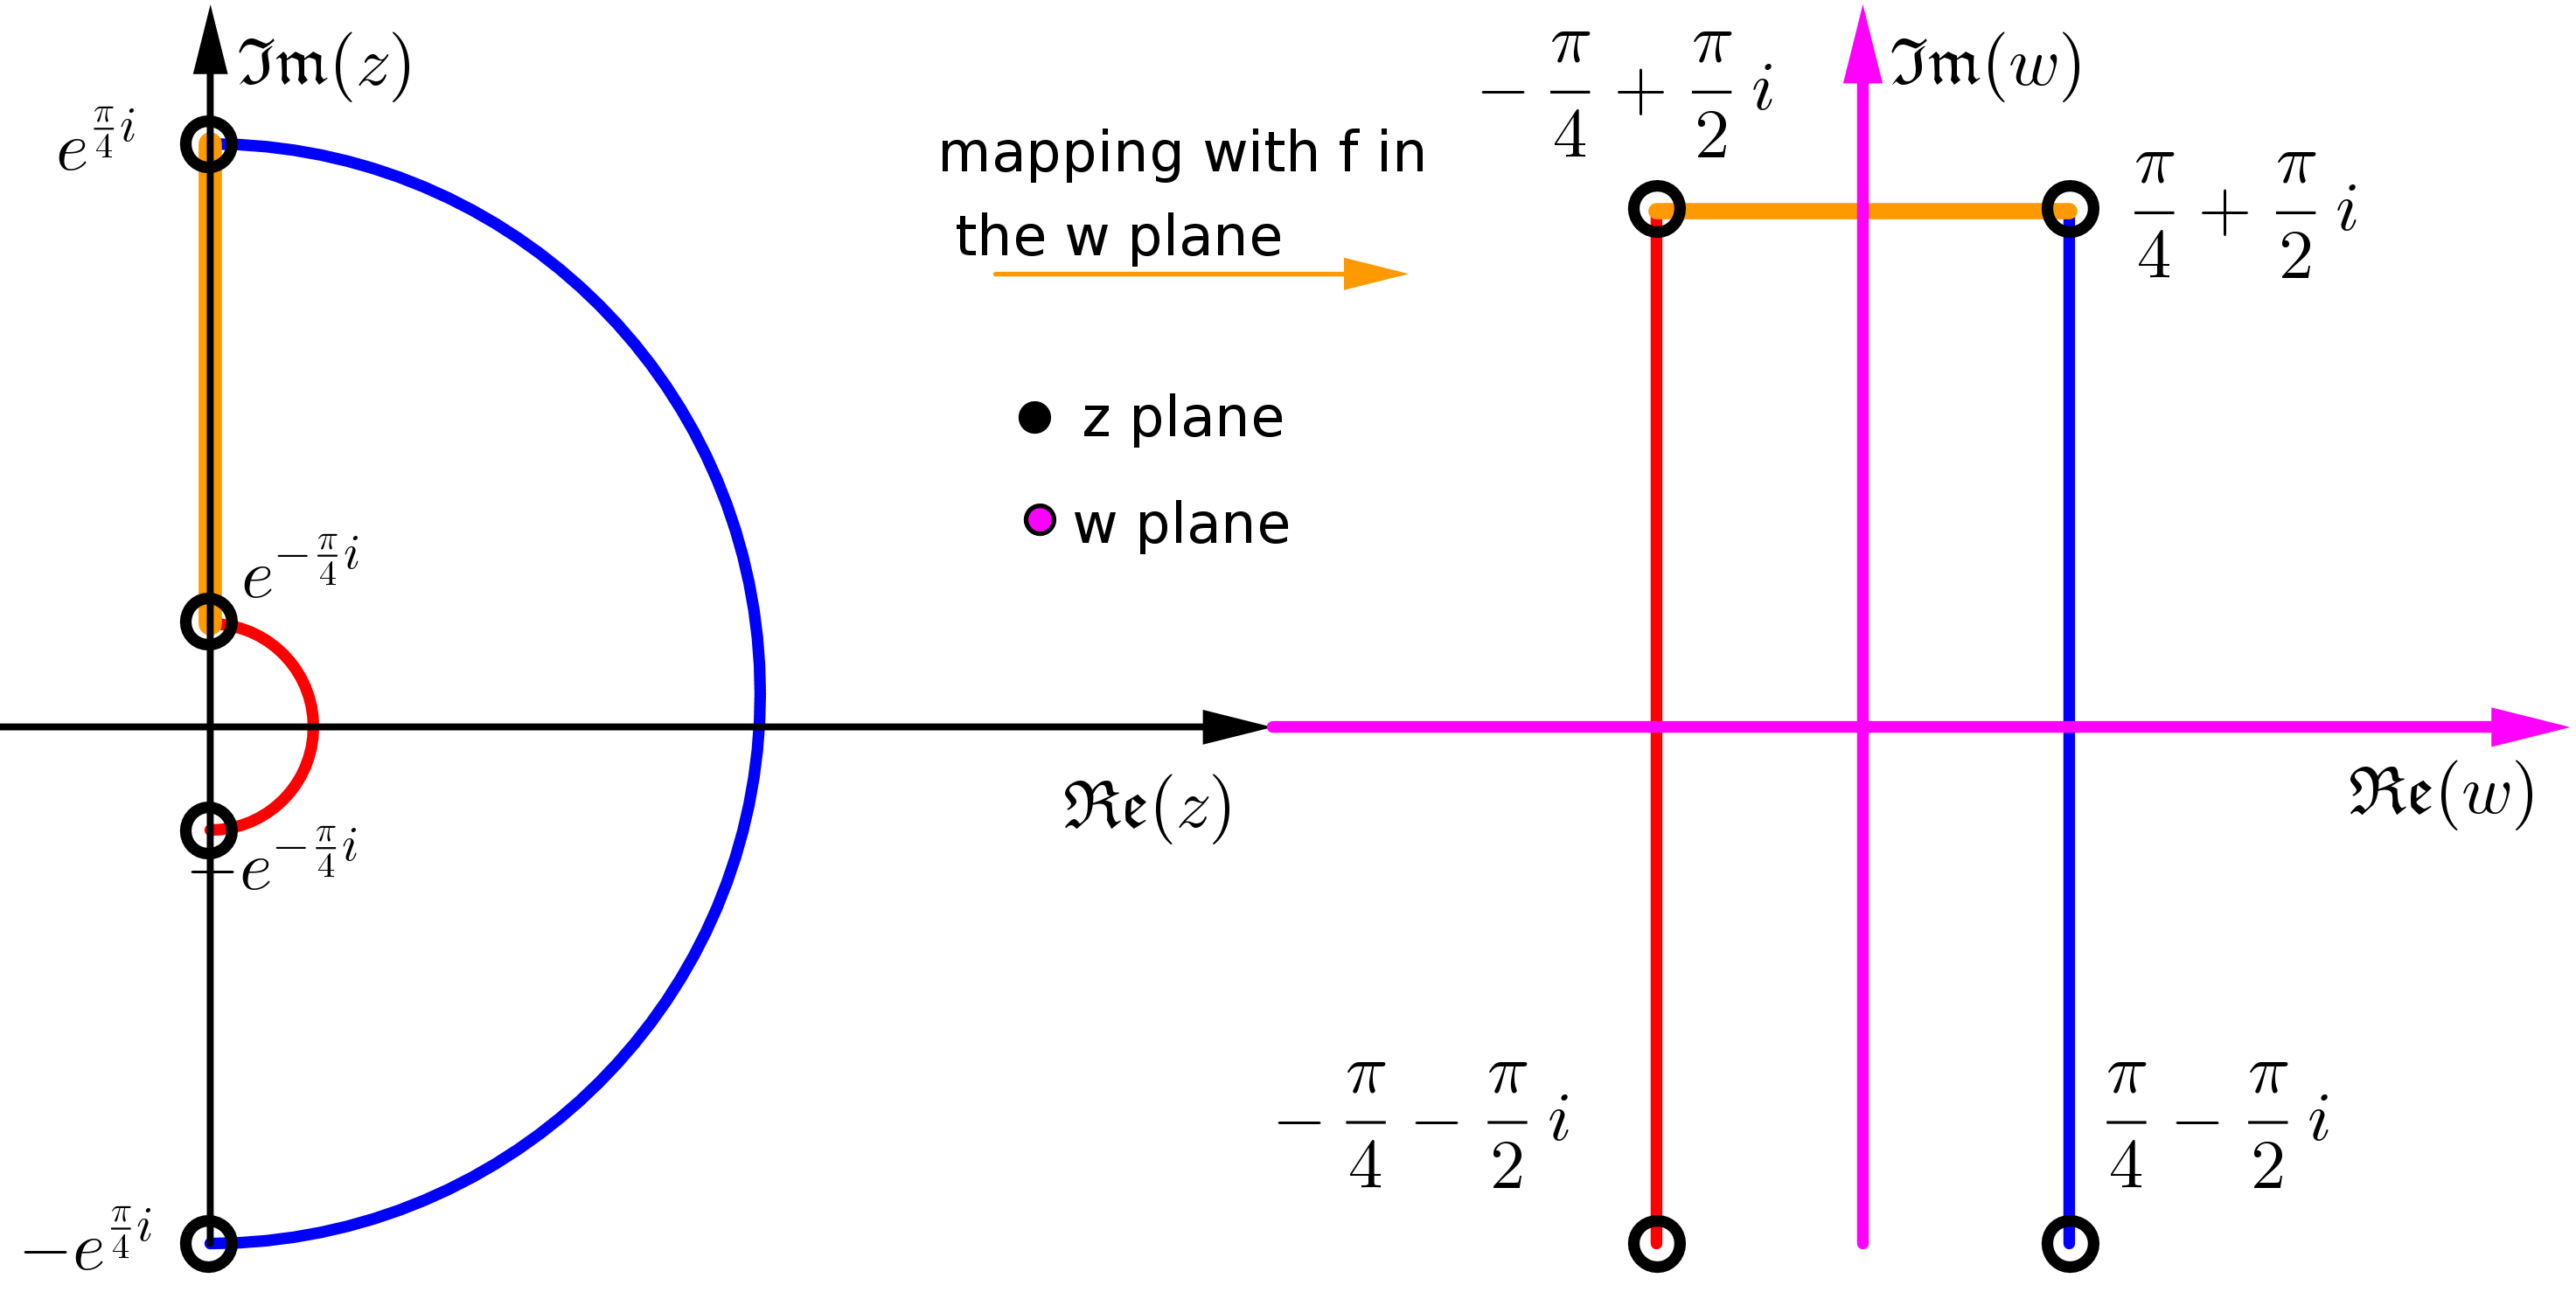
\includegraphics{2c.png}\end{center}
4.  The set 
$C_4=\left\{z\in\BBC\;\left|\;-\mathfrak{e}^{\frac{\pi}{4}}\leq\mathfrak{Im}
(z)\leq-\mathfrak { e }^{-\frac{\pi}{4}}, \mathfrak{Re}(z)=0
\right.\right\}$ is the vertical line segment which lies in the imaginary axis of the 
\textit{z-plane} with ending points (included) 
$\dsp z=-\mathfrak{e}^{-\frac{\pi}{4}}\mi$ and $\dsp z=-\mathfrak{e}^{\frac{\pi}{4}}\mi$. In this case $\dsp\textrm{Arg}(z)=-\frac{\pi}{2}$ 
and $\dsp\mathfrak{Re}(z)=0$, so \[\textrm{Log}(z)=\ln|y\cdot \mi|−\frac{\pi}{2}\mi=\ln⁡(y)−\mi\frac{\pi}{2}\]
which means that that the closed line segment $C_4$ is mapped under $f$ into the closed 
horizontal line line segment 
$\dsp t−\mi\frac{\pi}{2}$ with $t\in\left[-\frac{\pi}{4},\frac{\pi}{4}\right]$. In the next figure we see the green closed vertical line 
segment $C_4$ mapped into the green closed horizontal line segment of the \textit{w-plane}.
\begin{center}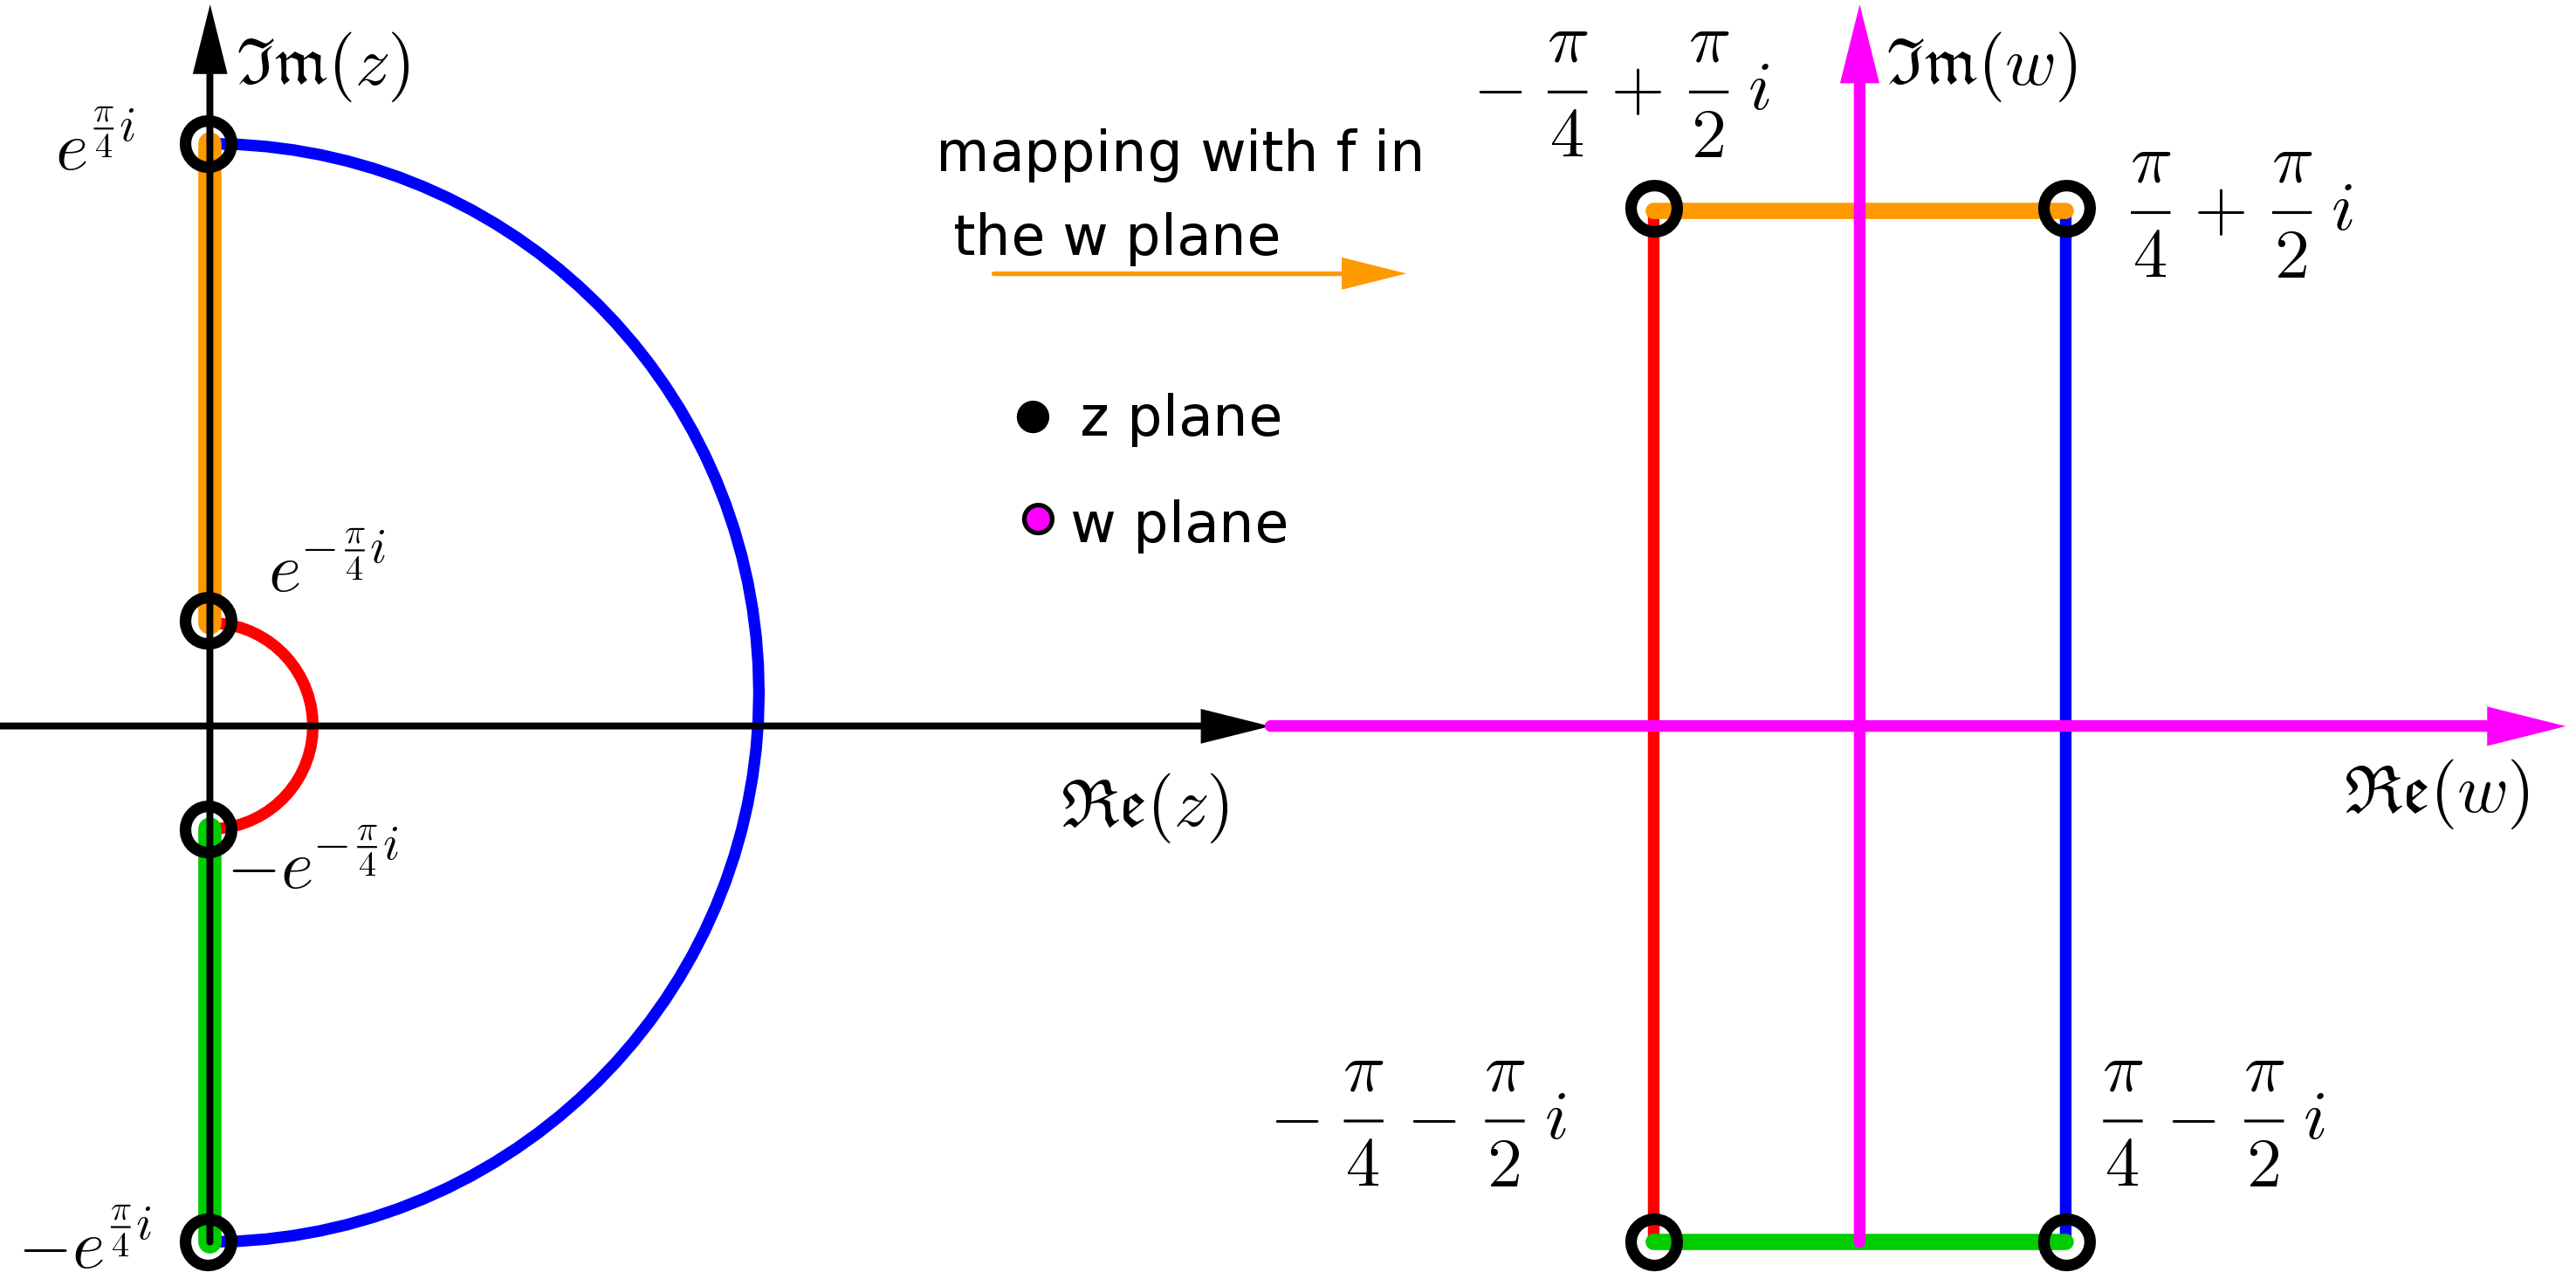
\includegraphics{2d.png}\end{center}
5. $\dsp A=\left\{z\in\BBC\left|\mathfrak{e}^{-\frac{\pi}{4}}<|z|<\mathfrak{e}^{\frac{\pi}{4}\mi},\mathfrak{Re}(z)>0\right.\right\}$ 
under $f$ is shown in the next figure.
\begin{center}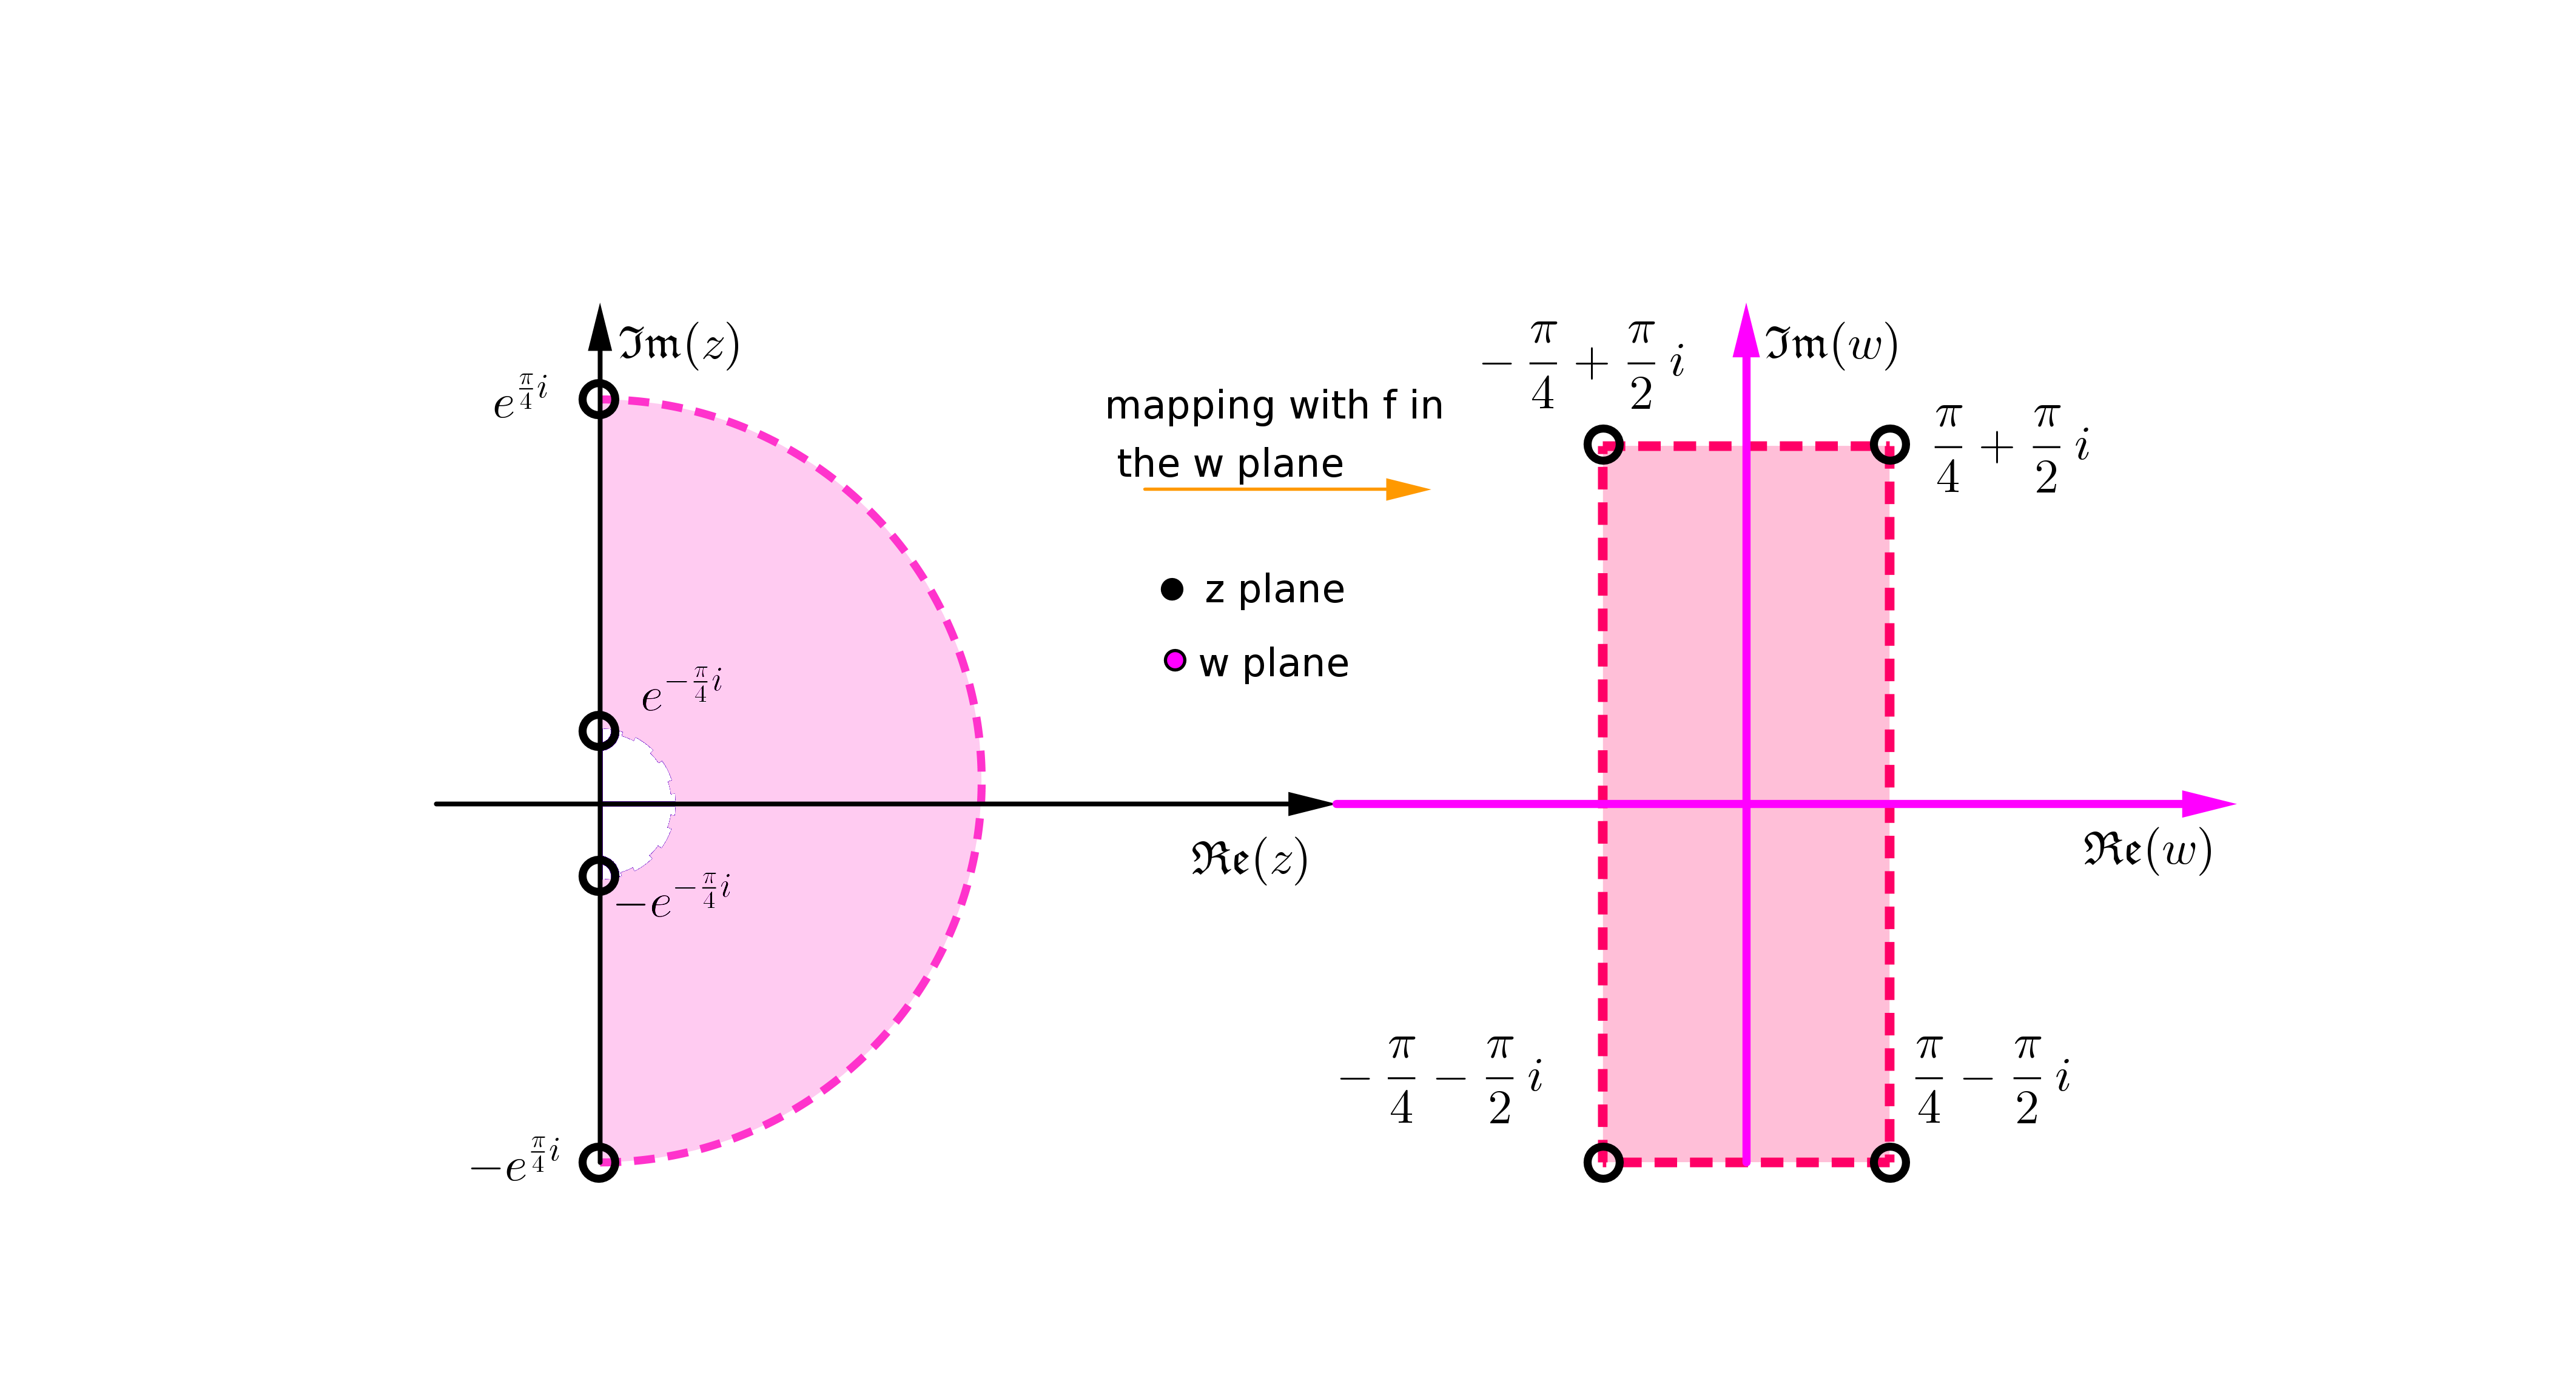
\includegraphics{2e.png}\end{center}

\definecolor{tcA}{rgb}{1,1,1}
\definecolor{tcB}{rgb}{1,0,0}
\definecolor{tcC}{rgb}{0,0,0}
\begin{center}
\begin{tabular}{l|l}
% use packages: color,colortbl
\rowcolor{tcA}
\textcolor{tcB}{- - - - - - - - - - - - -} & boundary not included\\
\rowcolor{tcA}
\textcolor{tcC}{O} & point not included
\end{tabular}
\end{center}
\textbf{2.} Let $f(z)=\sin(⁡z)$ and consider the domain $\dsp D=\left\{z\in\BBC\;\left| \;
0<\mathfrak{Re}(z)<\pi, 0<\mathfrak{Im}(z)<1\right.\right\}$ 
(an open rectangle). Find the maximum of $\dsp\left|f(z)\right|$ on $\dsp\overline{D}=D\bigcup\partial D$ as well as the z-value(s) at 
which $\dsp |f|$ attains this maximum value.
\begin{center}
 \textbf{Solution}
\end{center}
We want to find the maximum of $\dsp |f|$ over the rectangle $\dsp\overline{D}=D\bigcup\partial D$. From the maximum modulus 
principle the $\dsp \max_{z\in \overline{D}}\left|f(z)\right|$ is attained on the boundary $\partial D$. In next figure it is clear that 
we must seek for the maximum of $\dsp\left|f\right|$ on the lines $\dsp C_1, C_2, C_3, C_4$.
\begin{center}
\newrgbcolor{ffttff}{1 0.2 1}
\psset{xunit=1.0cm,yunit=1.0cm,algebraic=true,dotstyle=o,dotsize=3pt 
0,linewidth=0.8pt,arrowsize=3pt 2,arrowinset=0.25}
\begin{pspicture*}(-6.09,-2.63)(6.4,5.21)
\pspolygon[linewidth=2pt,linecolor=ffttff,fillcolor=ffttff,fillstyle=solid,opacity=0.25]
(-3.22,-0.7)(3.38,-0.7)(3.38,1.96)(-3.22,1.96)
\psline{->}(-3.22,-0.7)(4.8,-0.7)
\psline{->}(-3.22,-0.7)(-3.22,4.42)
\psline[linewidth=2pt,linecolor=ffttff](-3.22,-0.7)(3.38,-0.7)
\psline[linewidth=2pt,linecolor=ffttff](3.38,-0.7)(3.38,1.96)
\psline[linewidth=2pt,linecolor=ffttff](3.38,1.96)(-3.22,1.96)
\psline[linewidth=2pt,linecolor=ffttff](-3.22,1.96)(-3.22,-0.7)
\rput[tl](3.91,-0.75){$\mathfrak{Re}(z)$}
\rput[tl](-3.01,4.8){$\mathfrak{Im}(z)$}
\rput[tl](3.26,-0.62){$\pi$}
\rput[tl](-1.42,-0.84){$C_{1} = t$,with $t\in[0,\pi]$}
\rput[tl](-1.51,2.86){$C_{3} =t +\mi$,with $t \in[0,\pi]$}
\rput[lt](3.45,1.38){\parbox{4.11 cm}{$C_{2}=\pi +t\cdot\mi$,\\ with $t \in[0,1]$}}
\rput[lt](-5.67,1.46){\parbox{3.67 cm}{$C_{4}=t\cdot \mi$,\\ with $t \in[0,1]$}}
\rput[tl](-0.08,1.31){$\overline{D}$}
\begin{scriptsize}
\psdots[dotsize=7pt 0,dotstyle=*](-3.22,-0.7)
\psdots[dotsize=7pt 0,dotstyle=*](3.38,-0.7)
\psdots[dotsize=7pt 0,dotstyle=*](3.38,1.96)
\psdots[dotsize=7pt 0,dotstyle=*](-3.22,1.96)
\end{scriptsize}
\end{pspicture*}
\end{center}

Now will examine what happens on each line separately.\\
$\dsp C_1: \max_{z\in C_1}\sin⁡(z)=\max_{t\in [0,\pi]}\left|\sin⁡(t)\right|=\sin\left(\frac{\pi}{2}\right)=1$, attained at $\dsp z=\frac{\pi}{2}$.

$\dsp C_2: \max_{z\in C_2}\sin⁡(z)=\max_{t\in [0,1]}\sin⁡(\pi+t\mi)=\max_{t\in[0,1]}-\mi\sinh⁡(t)=\max_{t\in[0,1]}\sinh⁡(t)=\sinh⁡(1)$, 
attained at $z=\pi+\mi$.

$\dsp C_3: \sin⁡(x+y\mi)=\sin⁡(x)\cosh⁡(y)+\mi\cos⁡(x)\sinh⁡(y)$, so 
\begin{eqnarray*} \max_{z\in C_3}\sin⁡(z) &=&\max_{t\in [0,\pi]}\sin⁡(t)\cosh⁡(1)+\mi\cos⁡(t)\sinh⁡(1)\\ 
 &=&\max_{t\in[0,\pi]}\sqrt{\left(\sin⁡(t)\cosh⁡(1)\right)^{2}+\left(\cos⁡(t)\sinh⁡(1)\right)}^{2}\\
&=&\cosh(1)\end{eqnarray*} , attained at $\dsp z=\frac{\pi}{2}+\mi$.

$\dsp C_4: \max_{z\in C_{4}}\left|\sin(z)\right|=\max_{t\in\left[0,1\right]}\left|\sin(t\cdot \mi )\right|=\max_{t\in\left[0,1\right]}\left|\mi\cdot \sinh(t )\right|=\sinh(1)$, attained at $\dsp z=\mi$.

So summing up the above we get $\dsp\max_{z\in 
\overline{D}}\left|f(z)\right|=\left|f\left(\frac{\pi}{2}+\mi\right)
\right|=\cosh(1)$, which means that the \textbf{maximum} modulus of $f$ is 
$\dsp\cosh(1)$ attained at $\dsp z = \frac{\pi}{2}+\mi$.


$\dagger$ Recall that $\dsp\sinh⁡(z) =\frac{\mathfrak{e}^{z}-\mathfrak{e}^{-z}}{2}$ and $\dsp \cosh(z)=\frac{\mathfrak{e}^{z} + 
\mathfrak{e}^{-z}}{2}$.
\end{document}